\documentclass[onecolumn, draftclsnofoot,10pt, compsoc]{IEEEtran}
\usepackage{graphicx}
\usepackage{url}
\usepackage{setspace}
\usepackage{float}


\usepackage{geometry}
\geometry{textheight=9.5in, textwidth=7in}

% 1. Fill in these details
\def \CapstoneTeamName{		AKA Robotics}
\def \CapstoneTeamNumber{		13}
\def \GroupMemberOne{     Arthur Shing}
\def \GroupMemberTwo{			Kevin Talik}
\def \GroupMemberThree{   Anish Asrani}
\def \CapstoneProjectName{		How to Make an Effective Robot Comedian}
\def \CapstoneSponsorCompany{	Oregon State University}
\def \CapstoneSponsorPerson{		Heather Knight}

% 2. Uncomment the appropriate line below so that the document type works
\def \DocType{		%Problem Statement
				%Requirements Document
				%Technology Review
				%Design Document
				Progress Report
				}

\newcommand{\NameSigPair}[1]{\par
\makebox[2.75in][r]{#1} \hfil 	\makebox[3.25in]{\makebox[2.25in]{\hrulefill} \hfill		\makebox[.75in]{\hrulefill}}
\par\vspace{-12pt} \textit{\tiny\noindent
\makebox[2.75in]{} \hfil		\makebox[3.25in]{\makebox[2.25in][r]{Signature} \hfill	\makebox[.75in][r]{Date}}}}
% 3. If the document is not to be signed, uncomment the RENEWcommand below
\renewcommand{\NameSigPair}[1]{#1}

%%%%%%%%%%%%%%%%%%%%%%%%%%%%%%%%%%%%%%%
\begin{document}

\bstctlcite{IEEEexample:BSTcontrol}
\begin{titlepage}
    \pagenumbering{gobble}
    \begin{singlespace}
        \hfill
        % 4. If you have a logo, use this includegraphics command to put it on the coversheet.
        %\includegraphics[height=4cm]{CompanyLogo}
        \par\vspace{.2in}
        \centering
        \scshape{
            \huge CS Capstone \DocType \par
            {\large\today}\par
            \vspace{.5in}
            \textbf{\Huge\CapstoneProjectName}\par
            \vfill
            {\large Prepared for}\par
            \Huge \CapstoneSponsorCompany\par
            \vspace{5pt}
            {\Large\NameSigPair{\CapstoneSponsorPerson}\par}
            {\large Prepared by }\par
            Group\CapstoneTeamNumber\par
            % 5. comment out the line below this one if you do not wish to name your team
            \CapstoneTeamName\par
            \vspace{5pt}
            {\Large
                \NameSigPair{\GroupMemberOne}\par
                \NameSigPair{\GroupMemberTwo}\par
                \NameSigPair{\GroupMemberThree}\par
            }
            \vspace{20pt}
        }
        \begin{abstract}
Human-Robot interaction can learn a lot from stand-up comedy. A stand-up set has scripted jokes, statements that are predetermined,
as well as improvisational statements, that give the performance a sense of liveliness and character. A comedian can observe
an audience and improvise a delivery of a joke to connect the audience to the content. This makes the experience more authentic and
genuine for the observer. The purpose of this project is to to discover what makes an entertaining interaction by studying a robot that
performs comedy. We propose that a performance is enhanced when (1) the comedian interacts spontaneously with the audience,
(2) the comedian has and conveys a coherent, well-developed character, and (3) the comedian adapts its act to cater to an audience
based on their reaction. These propositions will be tested locally, remotely, and in a real stand-up setting.
	\end{abstract}
    \end{singlespace}
\end{titlepage}
\newpage
\pagenumbering{arabic}
\tableofcontents
% 7. uncomment this (if applicable). Consider adding a page break.
%\listoffigures
%\listoftables
\clearpage

% 8. now you write!
\section{Introduction/Problem}
A lot of the machines that surround us aren't very engaging to interact with. They serve their purpose, people get what they need, and the interaction is over. People do not consider robots as entities. That is the gap we are trying to close by performing stand-up comedy with a robot. Stand-up comedy is a casual and entertaining way for people to get more exposure to robots and see that robots are not just objects, but they are much more than that.

An effective robot comedian should be able to entertain the audience and generate laughs. We hypothesize that the effectiveness is dependent on three major aspects - crowd-work or the ability to integrate the audience in the performance, portraying a coherent and convincing character, and the ability to adapt the performance based on audience feedback. We will base our performances and studies around these three areas.

\section{Progress So Far}
We managed to get a lot more time to work with the robot over the past few weeks. This has helped us better understand how it works and what we can do with it.
We have managed to put together some simple comedy scripts and interactive sets that take into consideration the feedback from the audience using speech recognition. We perform a fair bit of animations with the robot as well.

\section{Week-by-week Summary}


\subsection{Week 1}
Nothing happened here. This was the first week of class, we got a general idea of how the class is supposed to work for the next year, and we started considering project preferences.

\subsection{Week 2}
We finally got our project, \textit{How to Make an Effective Robot Comedian}.  We got in touch with each other and set up a slack channel to communicate (akarobotics.slack.com). We also found a suitable time to work weekly and also set up a weekly meeting time with our client. We also began working on the problem statement.
\subsection{Week 3}
We set up a GitHub repository for the project, and wrote a rough draft of the problem statement. Our client meeting with Heather Knight was an introduction to the research that we would be performing. Heather explained what social robotics is to us, and our three research questions; Topic adaptation during a performance, crowd work, and characterization. Comedy is building a bond of trust with the audience, and conveying topics that break the audiences expectation. We started to learn how we would evaluate our components to our system. We initially had trouble figuring out how performance metrics would work, but our client helped us out with that. For homework, our client requested that we watch some comedy and bring some clips to the next meeting.
\subsection{Week 4}
We showed our problem statement rough draft to our client. Apparently we started off on the wrong foot, so we made major revisions. We also began to research and look at existing research on Human-Robot Interaction and humor. We started to learn the software Choregraphe, from which our robot is programmed. This week was an extreme learning opportunity with LaTeX.

\subsection{Week 5}
We worked on the requirements document. We discussed our problem statement with Kirsten. Our team started to draft our technical overview, and reviewing tools that could be used to develop or respective system in the robot comedian. Kevin looked at natural language processing tools, integrating them into the Choregraphe environment and implementing abstract state machines for conversation. We also wrote some sample scripts, and discovered how difficult it was to write jokes. As our problem statement had been pushed back because it needed major revisions, we were a little behind on the requirements document.
\subsection{Week 6}
We showed a rough draft of the requirements document to our client, Heather. We were still on the mostly wrong foot, so we made major revisions. Our instructors and TA began mentioning the difficulty of our project, which brought us some concern. We were unsure whether to write a literature review for our tech review or not. Our meetings with Heather are starting to get more elaborate. Now that we understand the tools, Heather started to show us more specific examples of how to implement animations for jokes, and the general joke writing process. During this phase, we started to gather metrics for how our jokes will be identified. We started to experiment with the audio sensors, and quickly realized that the NAO robot was not designed to listen to large crowds.
\subsection{Week 7}
We met the robot for the first time, and tried playing around with it in Choregraphe. We assigned research questions and began to branch off and work on our own individual sections of the project. We began to write more scripts. Kevin developed the Seed Joke, Middle content, and closing joke design for dynamic set performance with Heather. This is how the robot internally represents the performance.
\subsection{Week 8}
We worked on our tech reviews. We also tested early implementations of our respective research questions in Choregraphe. We learned how to animate the robot. Meetings with Heather during this phase of the project are dedicated to iterating through the animations and jokes that we have written so far. Technically, the writing process of comedy is different from the other work for this project, and it is interesting to write content for an entertainment audience. Heather helped us condense our text jokes so that the robot can be understood. We started to evaluate ambient movement during a joke, such as moving hands and nodding the head.
\subsection{Week 9}
We further developed and tested early implementations. Some of these were scrapped. We had trouble thinking of topics/subjects to write jokes about. We finished our tech reviews. Before we reflected on this term, we started to visualize what work we need to complete over the next two terms. Animating jokes is going to be the most time consuming task, so we need to have a large base for this. Upon looking at the tasks completed during this term, we determined what is going well, and how we need to progress into the next phases of the project. We are getting close to implementing.
\subsection{Week 10}
We wrote some comedy scripts for the robot. We synthesized the work that had been completed this term across our three research questions. For adaptation, Kevin filmed simple branching between two jokes that have different topics from simple audience input. Arthur developed robotic and humanoid versions of jokes to evaluate the importance of robot character. Anish further investigated ways to interact with the audience. We all filmed the work that had been completed, and how it relates to our system. We also made examples for crowd-work and adaptive topic selection. Our aim was to have something presentable for the progress report. We worked on the design document as well.


\section{Issues and Solutions}
One of the issues we have had so far is coming up with material to write for the robot. Unsurprisingly, being funny is not easy and a lot goes into making a reasonable script that works well with the robot and appeals to other people. Overcoming this will involve gaining a lot more experience with the robot, and exposure to different kinds of comedy.

Animating the robot can be tricky as well. Each keyframe needs to be stored in a timeline block and the animation needs to iterate through these frames at a reasonable rate. Push the animations too fast and the robot will topple over and fall flat on its face. Have the animations too slow, and it goes out of sync from the joke it is trying to say. Timing each word to correctly match the animation can be tedious and time-consuming. This will come down to practice and working more and more with the robot to get an idea of what "works" and what does not. The timeline is shown in Figure \ref{fig:timeline}.

\begin{figure}[H]
  \centering
  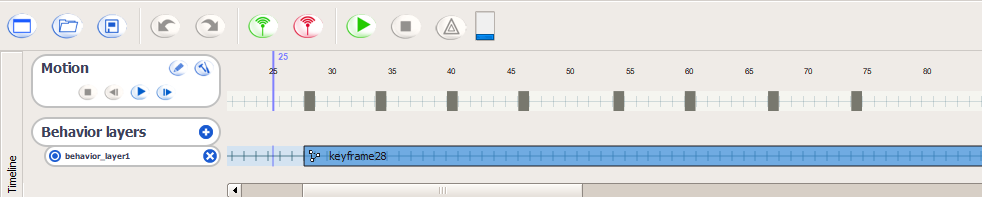
\includegraphics[width=0.75\textwidth,height=0.75\textheight,keepaspectratio]{timeline}
  \caption{The timeline frame of Choregraphe, used for animating with keyframes.}
	\label{fig:timeline}
\end{figure}

The voice recognition on the robot can be inconsistent sometimes. The range on the microphone isn't the greatest either. It will miss our cues completely at times, or go in a whole different direction.

While working on the robot, the robot needs breaks pretty regularly or it overheats. This can break the flow while testing and eliminates the possibility of longer performances/sets. There is not much we can do about it other than plan our scripts around the restrictions.

Outside the robot, one of the major issues we faced was writing documentation for the class as a research group.

\section{Retrospective}

Overall, this term, we have gotten a good grasp about the expectations from the project which were a little puzzling at the start of the term. We are starting to get the hang of our development environment - Choregraphe. Our understanding of the ins and outs of Choregraphe will only get better as we delve more into it. \\ \\

\begin{tabular}{|p{0.25\linewidth}|p{0.25\linewidth}|p{0.25\linewidth}|}
\hline
\centering  Positives &
\centering Deltas &
\centering Actions \tabularnewline
\hline

Starting to get a good grasp about project expectations &
Need to learn about people's comedy expectations &
Gain more exposure to different kinds of comedy and learn by some trial and error. \\
\hline
Becoming familiar with Choregraphe &
Need better jokes and better joke delivery &
Scripts will be rewritten \\
\hline



\end{tabular}

\pagebreak


% \bibliographystyle{IEEEtran}
% \bibliography{refs}

\end{document}
